\section{Optimizations}
\label{sec:design:optimizations}

There are two challenges in using CUDA virtual memory support for serving LLMs. First, invoking CUDA VMM APIs at runtime incurs high latency. Second, \cumemcreate currently allocates memory only at the granularity of large pages, i.e., multiples of 2MB. Use of large pages can waste physical memory due to internal fragmentation.  This section details a set of simple-yet-effective optimizations that we introduce to overcome these challenges.

\subsection{Hiding Latency of Memory Allocation}
The serving framework invokes the \vattnstep API in every iteration. The latency of \vattnstep depends on the number of page-groups that need to be mapped into \kvcache. Consider, for example, that the \kvcache of one request needs to be extended for \yimedium which has 60 layers. This requires 120 calls to \cumemmap + \cumemsetaccess each of which takes about 40 microseconds. Therefore, growing the \kvcache of one request by new page-groups (two per layer) adds about 5 millisecond latency to the corresponding iteration. The latency overhead grows proportional to the number of requests that need new page-groups in a given iteration. We propose the following optimizations to hide this latency:

\subsubsection{Overlapping memory allocation with compute (decode phase)}
We leverage the predictability of memory demand to overlap memory allocation with computation. In particular, note that each iteration produces a single output token for every decode request. Therefore, memory demand for a decode iteration is known ahead-of-time. Further, in the decode phase, a request requires at most one new page-group for each of its virtual tensors.  \sysname keeps track of the current context length and how much physical memory is already mapped for each request. Using this information, it determines when a request would need more memory and uses a background thread to allocate new page-groups when the preceding iteration is executing. For example, consider that a request \texttt{R1} would require more physical memory in iteration \texttt{i}. When the serving framework invokes \vattnstep API in iteration \texttt{i-1}, \sysname launches a background thread that maps page-groups for iteration \texttt{i}. Since per-iteration latency is typically in the range of 10s-100s of milliseconds, the background thread has enough time to prepare physical memory mappings for an iteration before it starts executing. This way, \sysname hides the latency of CUDA APIs by performing memory allocations out of the critical path. %Note that in every iteration, before returning execution control, the \vattnstep API must ensure that physical memory required in the \textit{current} iteration is already mapped. If the background thread launched in previous step is still active, the API waits for the thread to complete before returning (empirical observations suggest that synchronous wait almost never happens).



\subsubsection{Deferred reclamation + eager allocation (prefill phase)}
\label{sec:opt:defer}
We observe that allocating physical memory for the prefill phase can be avoided in many cases. Consider that a request \texttt{R1} completed in iteration \texttt{i} and a new request \texttt{R2} joins the running batch in iteration \texttt{i+1}. To avoid allocating page-groups to \texttt{R2} from scratch, \sysname simply defers the reclamation of \texttt{R1}'s page-groups (\autoref{fig:design:vattention}(d)) and assigns \texttt{R1}'s \reqid to \texttt{R2}. This way, \texttt{R2} uses the same tensors for its \kvcache that \texttt{R1} was using -- which are already backed by physical pages (\autoref{fig:design:vattention}(e)). Therefore, new allocations are required only if \texttt{R2}'s context length is higher than \texttt{R1}.

We further optimize the prefill phase by proactively allocating a small number of page-groups ahead of time. For this purpose, we try to keep a certain number of page-groups mapped into the virtual tensors of one of the inactive \reqid. When a new request arrives, we allocate this \reqid. At the same time, we identify a new \reqid to be allocated next and eagerly map physical page-groups for it. In most cases, these eager allocations obviate the need to allocate physical memory in the critical path of prefill execution. Finally, we trigger memory reclamation only when the number of page-groups cached in \sysname falls below a certain threshold (e.g., less than 10\% of GPU memory). We delegate both deferred reclamation and eager allocation to the background thread that the \vattnstep API spawns.

\begin{figure*}[t!]
    \centering
    \begin{subfigure}{0.33\textwidth}
    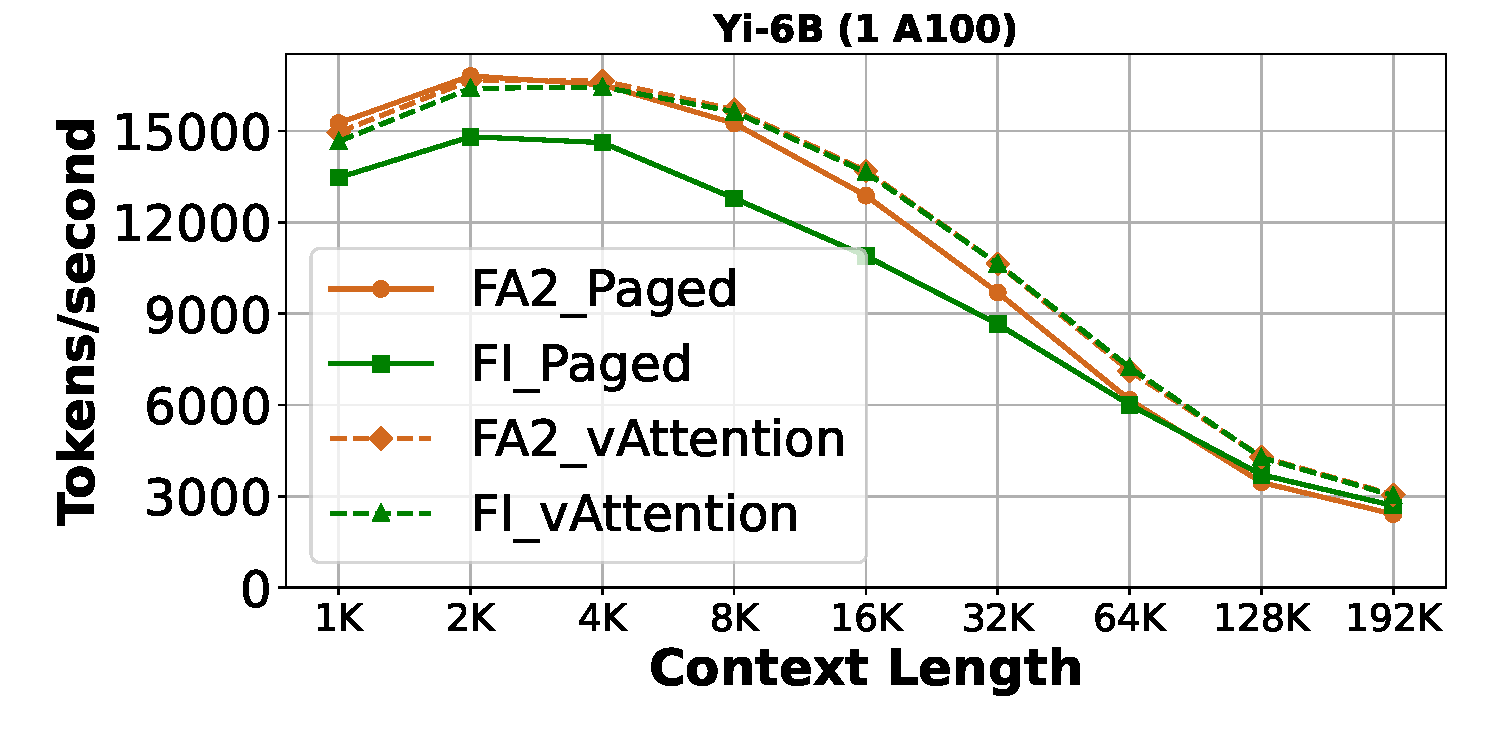
\includegraphics[trim={0 25 0 0}, clip=True, width=0.99\columnwidth]{graphs/eval_prefill_throughput/yi-6b-prefill-throughput.pdf} 
    \end{subfigure}
    \begin{subfigure}{0.33\textwidth}
    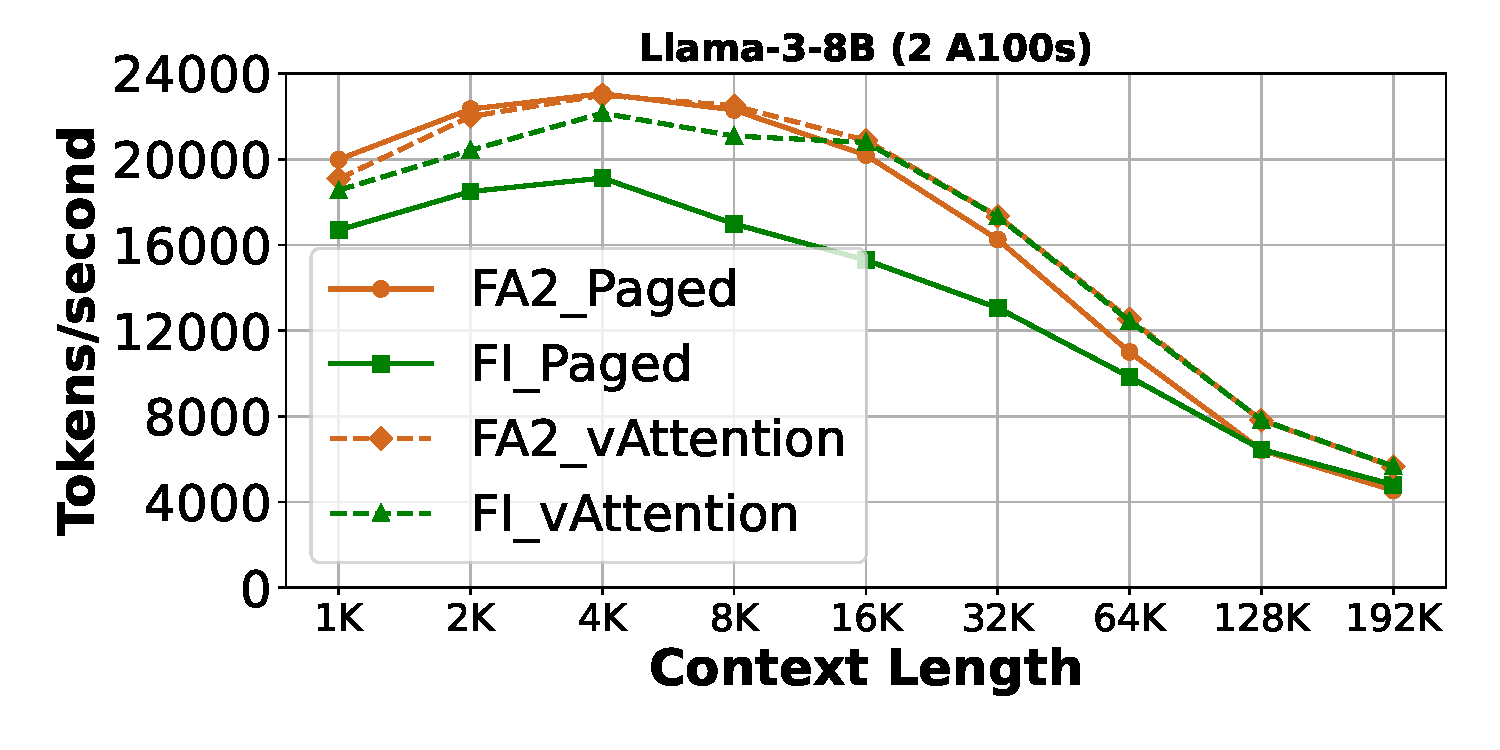
\includegraphics[trim={0 25 0 0}, clip=True, width=0.99\columnwidth]{graphs/eval_prefill_throughput/llama-3-8b-prefill-throughput.pdf}
    \end{subfigure}
    \begin{subfigure}{0.33\textwidth}
    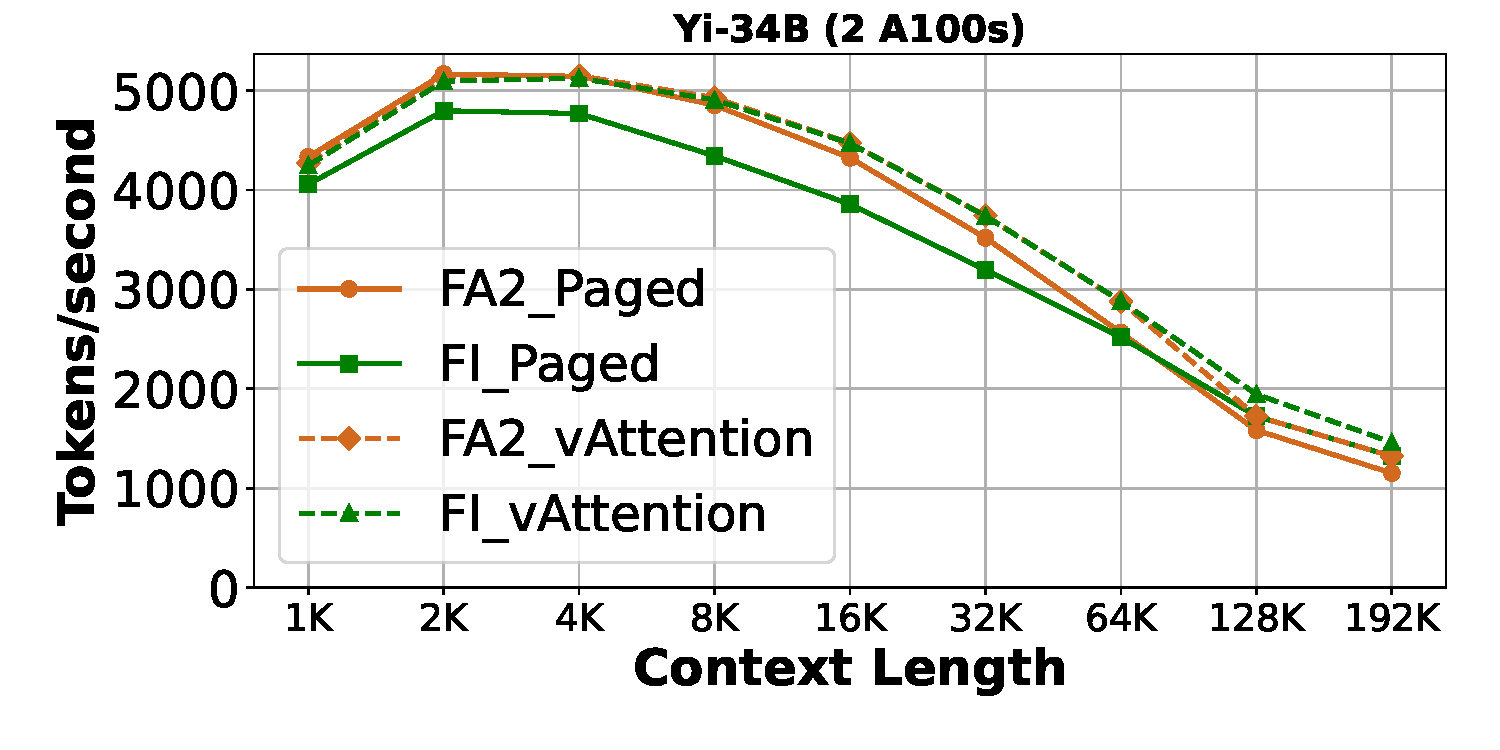
\includegraphics[trim={0 25 0 0}, clip=True, width=0.99\columnwidth]{graphs/eval_prefill_throughput/yi-34b-prefill-throughput.pdf}
    \end{subfigure}
    \caption{Prefill throughput. \sysname backed systems outperform the paged counterparts of both \flashattention and \flashinfer. Throughput for longer contexts is lower due to the quadratic complexity of prefill attention.}
    \label{fig:eval:prefill-throughput}
\end{figure*}


\subsection{Mitigating Internal Fragmentation}
\label{sec:opt:frag}

We mitigate internal fragmentation  by reducing the granularity of physical memory allocation. NVIDIA GPUs natively support at least three page sizes: 4KB, 64KB and 2MB~\cite{mcmgpus,gpu-mismanaged,gpu-reverse-engg-tlb1,pascalmmu}. Therefore, in principal, physical memory can be allocated in any multiple of 4KB sizes. The simplest way to achieve this would be to extend the existing CUDA VMM APIs (listed in \autoref{tab:design:cudaapis}) to also support allocating smaller pages (similar to how \texttt{mmap} in Linux supports multiple page sizes~\cite{ingens, hawkeye}). Unfortunately, the CUDA VMM APIs are implemented in the closed-source NVIDIA drivers which makes it impossible for us to modify their implementation. 

Fortunately, some part of NVIDIA drivers (particularly related to unified memory management) is open-source. Therefore, we implement a new set of APIs in the open-source NVIDIA drivers to mimic the same functionality that existing CUDA APIs provide but with support for multiple page sizes. The second column in \autoref{tab:design:cudaapis} shows our new APIs: most of our APIs have a one-to-one relationship with existing CUDA APIs except for \vmemmap that combines the functionality of \cumemmap and \cumemsetaccess, and \vmemrelease that combines the functionality of \cumemunmap and \cumemrelease for simplicity. In contrast to CUDA VMM APIs, our APIs allocate physical memory in 64KB, 128KB and 256KB sized page-groups. A serving framework can configure a desired page-group size in \sysname while initializing it (we use the standard 2MB pages if the configured page-group size is 2MB). \autoref{tab:design:cudaapis} shows the latency of each API with different page-group sizes.